\documentclass{article}
\usepackage{ulem}
\usepackage{amsmath}
\usepackage[pdftex]{graphicx}   
\title{\bf{Fluid Mechanics}}
\author{Nicholas Malaya} \date{}

\begin{document}
\maketitle


%%%%%%%%%%%%%%%%%%%%%%%%%%%%%%%%%%%%%%%%%%%%%%%%%
%
%        Introduction
%
%%%%%%%%%%%%%%%%%%%%%%%%%%%%%%%%%%%%%%%%%%%%%%%%%
\newpage
\section{Introduction}

Shear stress
\begin{equation}
    \tau = \mu\frac{du}{dy}
\end{equation}
\newline
\newline
Dynamic ($\mu$) and Kinematic ($\nu$) viscosity
\begin{equation}
  \nu \equiv \frac{\mu}{\rho}
\end{equation}
\newline
\newline
Specific Gravity
\begin{equation}
  SG \equiv \frac{\rho}{\rho_\text{water at 4$^\circ$C}}
\end{equation}

%%%%%%%%%%%%%%%%%%%%%%%%%%%%%%%%%%%%%%%%%%%%%%%%%
%
%        Fluid Statics
%
%%%%%%%%%%%%%%%%%%%%%%%%%%%%%%%%%%%%%%%%%%%%%%%%%
\section{Fluid Statics}

Incompressible fluid at rest
\begin{equation}
    p_1-p_2 = \gamma (z_2-z_1)
\end{equation}
\newline
\newline
Pressure head
\begin{equation}
    h = \frac{p_1-p_2}{\gamma}
\end{equation}
\newline
\newline
Buoyant force ($V$ is volume)
\begin{equation}
    F_B = \gamma_{fluid} V
\end{equation}
\newline
\newline
Circulation: denotes the net algebraic strength of all the vortex filaments contained within the closed curve
\begin{equation}
  \Gamma = \oint_{C} Vcos\alpha ds
\end{equation}
\newline
\newline
Vorticity: 2 times the angular velocity. Equal to zero for irrotational flows.
\begin{equation}
  \mathbf{\zeta} = 2\mathbf{\omega} = curl\mathbf{V}
\end{equation}


%%%%%%%%%%%%%%%%%%%%%%%%%%%%%%%%%%%%%%%%%%%%%%%%%
%
%        Elementary Fluid Dynamics
%
%%%%%%%%%%%%%%%%%%%%%%%%%%%%%%%%%%%%%%%%%%%%%%%%%
\newpage
\section{Elementary Fluid Dynamics}

Streamlines - lines that are tangent to the velocity vectors throughout the flow field
\newline
\newline
Bernoulli (for assumptions remember ISIS: inviscid, steady, incompressible, on a streamline). Bernoulli can only be used across streamlines if the flow is irrotational.
\begin{equation}
  \frac{v^2}{2}+gz+\frac{p}{\rho}=constant
\end{equation}
We advance the non-linear terms explicitly. The linear terms implicitly. The linear terms are the viscous operator. 
\newline
\newline
Across the streamline
\begin{equation}
    p + \rho\int\frac{V^2}{R}dn + \gamma z = constant
\end{equation}
\newline
\newline
Static pressure - actual thermodynamic pressure of the fluid as it flows, measured by pressure tap on a flat surface
\newline
\newline
Dynamic pressure - $\rho V^2/2$, measured by inserting a tap pointing upstream
\newline
\newline
Stagnation pressure - static pressure plus dynamic pressure
\newline
\newline
Total pressure - Bernoulli equation, static plus dynamic plus hydrostatic.
\newline
\newline
Flow through a flow meter Eq 3.20
\begin{equation}
    Q = A_2\sqrt\frac{2(p_1-p_2)}{\rho[1-(A_2/A_1)^2]}
\end{equation}


%%%%%%%%%%%%%%%%%%%%%%%%%%%%%%%%%%%%%%%%%%%%%%%%%
%
%        Fluid Kinematics
%
%%%%%%%%%%%%%%%%%%%%%%%%%%%%%%%%%%%%%%%%%%%%%%%%%
\newpage
\section{Fluid Kinematics}

2D streamline 
\begin{equation}
    \frac{dy}{dx}=\frac{v}{u}
\end{equation}
\newline
\newline
Material derivative
\begin{equation}
    \frac{D()}{Dt} = \frac{\partial()}{\partial t} + u\frac{\partial()}{\partial x} + v\frac{\partial()}{\partial y} + w\frac{\partial()}{\partial z}
\end{equation}
\newline
\newline
Acceleration (the portion represented by the spatial derivatives is the convective acceleration)
\begin{equation}
    \mathbf{a} = \frac{\partial\mathbf{V}}{\partial t} + u\frac{\partial\mathbf{V}}{\partial x} + v\frac{\partial\mathbf{V}}{\partial y} + w\frac{\partial\mathbf{V}}{\partial z}
\end{equation}
\newline
\newline
Reynolds Transport Theorem (p 170-177) ($V$ is volume)
\begin{equation}
    B=mb
\end{equation}
\begin{equation}
    \frac{dB_{cv}}{dt}=\frac{d}{dt}\left(\int_{cv}\rho b dV\right)
\end{equation}

    

%%%%%%%%%%%%%%%%%%%%%%%%%%%%%%%%%%%%%%%%%%%%%%%%%
%
%        Finite Control Volume Analysis
%
%%%%%%%%%%%%%%%%%%%%%%%%%%%%%%%%%%%%%%%%%%%%%%%%%
\newpage
\section{Finite Control Volume Analysis}

Continuity Integral Form (for a deforming CV the time rate of change term is usually nonzero)
\begin{equation}
    \frac{\partial}{\partial t}\int_{cv}\rho d\sout{V} + \int_{cv}\rho \mathbf{V}\cdot \mathbf{\hat{n}} dA = 0
\end{equation}
\newline
\newline
Moving CV continuity
\begin{equation}
    \mathbf{V} = \mathbf{W} + \mathbf{V}_{cv}
\end{equation}
\noindent where $W$ is the relative velocity, $V_{cv}$ is the velocity of the control volume, and $V$ is the absolute velocity of the fluid.
\begin{equation}
     \frac{\partial}{\partial t}\int_{cv}\rho d\sout{V} + \int_{cv}\rho \mathbf{W}\cdot \mathbf{\hat{n}} dA = 0
\end{equation}
\newline
\newline
Linear momentum 
\begin{equation}
    \frac{\partial}{\partial t}\int_{cv}\mathbf{V}\rho d\sout{V} + \int_{cv}\mathbf{V}\rho \mathbf{V}\cdot \mathbf{\hat{n}} dA = \sum\mathbf{F}
\end{equation}
\newline
\newline
Linear momentum for a moving CV
\begin{equation}
    \int_{cs}\mathbf{W}\rho\mathbf{W}\cdot \mathbf{\hat{n}} dA = \sum\mathbf{F}
\end{equation}
\newline
\newline
Momentum of momentum 
\begin{equation}
    \frac{\partial}{\partial t}\int_{cv}(\mathbf{r}\times\mathbf{V})\rho d\sout{V} + \int_{cv}(\mathbf{r}\times\mathbf{V})\rho \mathbf{V}\cdot \mathbf{\hat{n}} dA = \sum(\mathbf{r}\times\mathbf{F})
\end{equation}
\newline
\newline
Energy integral from Eq 5.64
\begin{equation}
  \frac{\partial}{\partial t} \int_\text{cv} e \rho d V + \int_\text{cs} \left(\hat{h} + \frac{V^2}{2} + g z\right) \rho \mathbf{V} \mathbf{\cdot} \mathbf{\hat{n}} d A = \dot{Q}_\text{net,in} - \dot{W}_\text{shaft,net out}
\end{equation}
% \begin{equation}
%  \frac{d}{dt}\int_{\Omega(t)} T(x,t) dV = \int_{\Omega} \frac{\partial}{\partial t} T dV + \int_{\partial \Omega} \hat n \cdot w T dA = \int_{\Omega}\frac{\partial}{\partial t} T + \nabla \cdot w T dV
% \end{equation}
\newline
\newline
Kinetic energy coefficient
\begin{equation}
  \alpha = \frac{\int_A (V^2/2) \rho \mathbf{V}dA \cdot \mathbf{\hat{n}}}{\dot{m} \overline{V}^2/2}
\end{equation}
\newline
\newline
Energy w/ head loss and kinetic energy coefficients Eq 5.89
\begin{equation}
    \frac{p_o}{\gamma} + \frac{\alpha_o\bar{V}^2_o}{2g}+z_o = \frac{p_i}{\gamma} + \frac{\alpha_i\bar{V}^2_i}{2g}+z_i + \frac{W_{shaft,in}}{g} - h_L
\end{equation}

%%%%%%%%%%%%%%%%%%%%%%%%%%%%%%%%%%%%%%%%%%%%%%%%%
%
%        Differential Analysis of Fluid Flow
%
%%%%%%%%%%%%%%%%%%%%%%%%%%%%%%%%%%%%%%%%%%%%%%%%%
\newpage
\section{Differential Analysis of Fluid Flow}

Hydraulic diameter
\begin{equation}
  D_h = \frac{4A_c}{P}
\end{equation}
\newline
\newline
Conservation of Mass
\begin{equation}
  \frac{\partial\rho}{\partial t} + \frac{\partial\rho u}{\partial x} +\frac{\partial\rho v}{\partial y} +\frac{\partial\rho w}{\partial z} = 0
\end{equation}
\newline
\newline
Streamfunction
\begin{equation}
  u=\frac{\partial\psi}{\partial y}\quad v=-\frac{\partial\psi}{\partial x}
\end{equation}
\newline
\newline
Relation between complete and viscous stress tensor for Newtonian fluids
\begin{equation}
  \sigma_{ij} = \tau_{ij} - p \delta_{ij}
\end{equation}
\newline
\newline
N-S equation

Vector
\begin{equation}
  \rho\frac{D\mathbf{V}}{Dt} = -\nabla p + \rho\mathbf{g} + \mu \nabla^2\mathbf{V}
\end{equation}

Cartesian x
\begin{equation}
  \rho\left( \frac{\partial u}{\partial t} + u\frac{\partial u}{\partial x} + v\frac{\partial u}{\partial y} + w\frac{\partial u}{\partial z}\right) = -\frac{\partial p}{\partial x} + \rho g_x + \mu\left( \frac{\partial^2 u}{\partial x^2} + \frac{\partial^2 u}{\partial y^2} + \frac{\partial^2 u}{\partial z^2}\right)
\end{equation}
%%%%%%%%%%%%%%%%%%%%%%%%%%%%%%%%%%%%%%%%%%%%%%%%%
%
%        Similitude, Dimensional Analysis, and Modeling
%
%%%%%%%%%%%%%%%%%%%%%%%%%%%%%%%%%%%%%%%%%%%%%%%%%
\newpage
\section{Similitude, Dimensional Analysis, and Modeling}

Buckingham Pi Theorem: If an equation involving $k$ variables is dimensionally homogeneous, it can be reduced to a relationship amount $k - r$ independent dimensionless products, where $r$ is the rank of the dimensional matrix (the minimum number of reference dimensions required to describe the variables).


%%%%%%%%%%%%%%%%%%%%%%%%%%%%%%%%%%%%%%%%%%%%%%%%%
%
%        Viscous Flow in Pipes
%
%%%%%%%%%%%%%%%%%%%%%%%%%%%%%%%%%%%%%%%%%%%%%%%%%
\newpage
\section{Viscous Flow in Pipes}

Pipe flow in a round pipe is laminar for around $Re_D < 2100$. The flow is turbulent for approximately $Re_D > 4000$.
\newline
\newline
Turbulent entry length for $10^4 < Re_D < 10^5$: $20 < l_e / D < 30$
\newline
\newline
Derive viscous stress as a function of pressure gradient from N-S equations
critical tube $Re_D$ (p. 404, 5th ed.)
\newline
\newline
Darcy friction factor (in terms of pressure drop and shear stress) (p. 415, 5th ed)
\begin{equation}
  f = \frac{\Delta p D \rho V^2}{2l}
\end{equation}
\begin{equation}
  f = \frac{64}{Re}\quad\text{laminar}
\end{equation}
\newline
\newline
Laminar velocity profile in a tube
\begin{equation}
  u = \frac{r_0^2}{4 \mu} \left(- \frac{d p}{d x}\right) \left(1 - \frac{r^2}{r_0^2}\right)
\end{equation}
\newline
\newline
Reynolds stress (p. 423, 5th ed.)
\newline
\newline
Friction Velocity (ch. 8 p 425)
\begin{equation}
  u_\tau = \sqrt{\frac{\tau_w}{\rho}}
\end{equation}
\newline
\newline
The reynolds stress tensor is the stress in a fluid due to the random turbulent fluctuations in the fluid momentum (ch. 8):
\begin{equation}
  \rho \overline{u'_i u'_j}
\end{equation}
\newline
\newline
Losses in pipes:

Major losses
\begin{equation}
  h_{L,major} = f\frac{l}{D}\frac{V^2}{2g}
\end{equation}

Minor losses
\begin{equation}
  h_{L,minor} = K_L\frac{V^2}{2g}\quad \Delta p = K_L 0.5\rho V^2
\end{equation}

%%%%%%%%%%%%%%%%%%%%%%%%%%%%%%%%%%%%%%%%%%%%%%%%%
%
%        Flow Over Immersed Bodies
%
%%%%%%%%%%%%%%%%%%%%%%%%%%%%%%%%%%%%%%%%%%%%%%%%%
\newpage
\section{Flow Over Immersed Bodies}

Derive Displacement Thickness
\begin{equation}
  \delta^* = \int_0^\delta (1-\frac{u}{U})dy
\end{equation}
\newline
\newline
Derive Momentum Thickness. The momentum thickness is transverse distance by which the boundary should be displaced to compensate for the reduction in momentum of the flowing fluid on account of boundary layer formation. (ch. 9)
\begin{equation}
  \Theta = \int_0^\delta \frac{u}{U}(1-\frac{u}{U})dy
\end{equation}
\newline
\newline
Derive Boundary Layer Equations from N-S with the assumptions:
\begin{equation}
  \frac{\partial^2 u}{\partial x^2} \ll \frac{\partial^2 u}{\partial y^2}
\end{equation}
\begin{equation}
  v \ll u\quad\text{and}\quad\frac{\partial}{\partial x} \ll \frac{\partial}{\partial y}
\end{equation}
\begin{equation}
  \frac{\partial p}{\partial x} \approx \frac{\partial p_\infty}{\partial x}
\end{equation}
\newline
\newline
Laminar boundary layer equations: 
\begin{equation}
  \frac{\partial u}{\partial x} + \frac{\partial v}{\partial y} = 0
\end{equation}
\begin{equation}
  u\frac{\partial u}{\partial x} + v\frac{\partial u}{\partial y} = -\frac{\partial p}{\partial x} + \mu\frac{\partial^2 u}{\partial y^2}
\end{equation}
where
\begin{equation}
  -\frac{d p}{d x} = U \frac{d U}{d x}
\end{equation}
\newline
\newline
Laminar BL thickness proportionality. (constant is 5 for Blausius solution)
\begin{equation}
  \delta \sim C\left(\frac{\nu x}{U}\right)^{1/2}
\end{equation}
\newline
\newline
Blausius Solution:
\begin{equation}
  \eta=\frac{y}{\delta}=y(U/\nu x)^{1/2}\quad\frac{u}{U}=f'(\eta)\quad\psi = \sqrt{U\nu x}f(\eta)
\end{equation}
\begin{equation}
  2 \frac{\text{d}^3 f}{\text{d} \eta^3} + f \frac{\text{d}^2 f}{\text{d} \eta^2} = 0
\end{equation}
Local friction coefficient for Blausius solution
\begin{equation}
  c_\text{f,x} = 0.664 Re_x^{-1/2}
\end{equation}
\newline
\newline
Momentum thickness and drag force relations
\begin{equation}
  \frac{dD}{dx} = b \tau_w
\end{equation}
\begin{equation}
  D = \rho b U^2 \Theta
\end{equation}
\begin{equation}
  \tau_\text{w} = \rho U^2 \frac{d \Theta}{d x}
\end{equation}
\newline
\newline
Local friction coefficient
\begin{equation}
  c_f = \frac{2\tau_w}{\rho U^2}
\end{equation}
\begin{equation}
  C_{Df} = \frac{1}{l}\int_0^l c_f dx
\end{equation}
\newline
\newline
Approximate transitional value of $Re_x$ for flow over a flat plate is $\approx 5 \cdot 10^5$
Boundary layer separation occurs when the fluid at the surface lacks the momentum to overcome the adverse ($dp/dx > 0$) pressure gradient. The turbulent boundary layer has more momentum than the laminar boundary layer and thus delays separation.
\newline
\newline
Von Karman momentum integral
\begin{equation}
  \frac{\tau_w}{\rho} =  \frac{d}{dx}(U^2\Theta) + \delta^* U\frac{dU}{dx}
\end{equation}
Drag. Friction Drag from shear and Form Drag from pressure. 
\begin{equation}
  F_D = \frac{1}{2}\rho v^2 C_D A
\end{equation}
\newline
\newline
Lift
\begin{equation}
  F_L = \frac{1}{2}\rho v^2 C_L A
\end{equation}
\newline
\newline
Pressure coefficient
\begin{equation}
  C_p = \frac{p-p_\infty}{\frac{1}{2}\rho_\infty U^2_\infty}
\end{equation}
\newline
\newline
Sketch lift and drag curves for spheres/cylinders and airfoils
\begin{figure}[!ht]
\centering
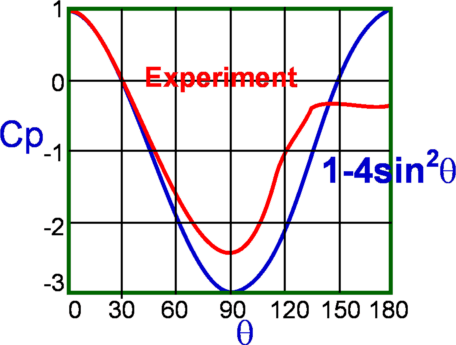
\includegraphics[width=0.6\textwidth]{./Figures/cpdist}
\caption{Pressure coefficient $C_p$ for a cylinder in cross-flow.}
\end{figure}
\begin{figure}[!ht]
\centering
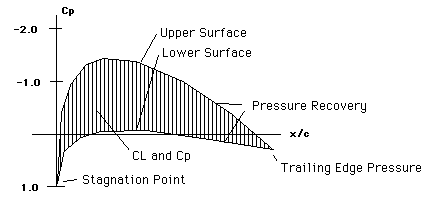
\includegraphics[width=0.75\textwidth]{./Figures/AirfoilCp}
\caption{Pressure coefficient $C_p$ for an airfoil.}
\end{figure}
\begin{figure}[!ht]
\centering
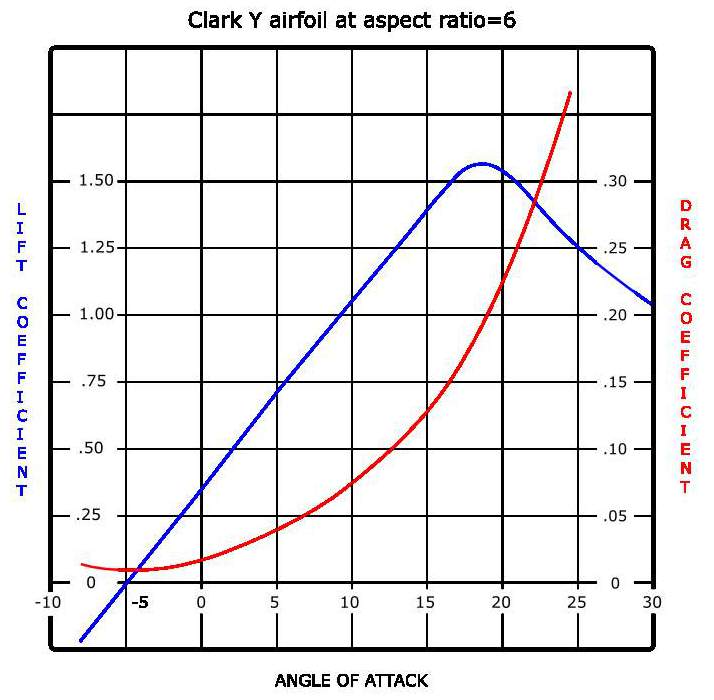
\includegraphics[width=0.6\textwidth]{./Figures/Lift_drag_graph}
\caption{Lift and drag coefficients for an airfoil.}
\end{figure}
\newline
\newline
Purpose of flaps on an airplane:

Deployed flaps increase $C_\text{L}$ but at the expense of also increasing $C_\text{D}$. This is actually a good condition during landing. A decrease in speed requires larger lift to sustain flight and the increase in drag helps to further slow down the plane.
\clearpage

%%%%%%%%%%%%%%%%%%%%%%%%%%%%%%%%%%%%%%%%%%%%%%%%%
%
%        Compressible Flow
%
%%%%%%%%%%%%%%%%%%%%%%%%%%%%%%%%%%%%%%%%%%%%%%%%%
\newpage
\section{Compressible Flow}

Isentropic Relations
\newline
\newline
Speed of sound for an isotropic perfect gas
\begin{equation}
  c^2 = \left(\frac{\partial p}{\partial \rho}\right)_s
\end{equation}
\begin{equation}
  p = \text{const.} \rho^\gamma
\end{equation}
\begin{equation}
  c^2 = \frac{\gamma p}{\rho} = \gamma R T
\end{equation}
\newline
\newline
Single-phase continuity
\begin{equation}
  \frac{\partial \rho}{\partial t} + \frac{\partial \rho u_i}{\partial x_i} = 0
\end{equation}
\newline
\newline
Mach Number
\begin{equation}
  Ma \equiv \frac{u}{c}
\end{equation}
\newline
\newline
A perfect gas may not be considered incompressible for $Ma > 0.3$.

%%%%%%%%%%%%%%%%%%%%%%%%%%%%%%%%%%%%%%%%%%%%%%%%%
%
%        Dimensionless Numbers
%
%%%%%%%%%%%%%%%%%%%%%%%%%%%%%%%%%%%%%%%%%%%%%%%%%
\newpage
\section{Dimensionless Numbers}
Schmidt Number:
\begin{equation}
  Sc = \frac{\nu}{D}
\end{equation}
The ratio of momentum diffusivity (viscosity) and mass diffusivity
\newline
\newline
Damkohler Number
\begin{equation}
  Da = \frac{\textrm{fluid time}}{\textrm{chemical reaction time}}
\end{equation}
\newline
\newline
Knudson Number
\begin{equation}
  Kn = \frac{\lambda}{L}
\end{equation}

\newpage
Amat victoria curam. 

\end{document}
